\section{The sample}
\label{sec:sample}

This search covers \NWindows{} spectral windows toward \NStars{}
stars in \NSystems{} systems within 40\,pc, drawn from \NEB{}
public ALMA execution blocks and \TotalDataTB\,TB of raw data through one
frozen pipeline, \StTelHours\,h of telescope time and \LdgCensusHours\,h
summed over windows. We call that set the
\emph{primary census}, and it is the set every limit, every crossing and
every expectation in this paper is computed over. Four further sets of blocks
enter the paper and none of them is part of it: a hold-out of \LdgHoldEB{}
blocks and \LdgHoldWin{} windows, reserved before any block on its own side
of the rule was searched; an archival extension of \LdgExtEB{} blocks and
\LdgExtWin{} windows, searched afterwards; an out-of-sample control beyond
40\,pc; and an external sample used only to calibrate the spatial statistic.
Table~\ref{tab:blockledger} gives all five sets in rows that sum, with the
results each one enters; wherever a number in this paper is computed over
something other than the primary census, that table's name for it is used at
the point of use.

Three words are not interchangeable here. A \emph{star} is one stellar
component, a \emph{system} a bound group counted once however many of its
components were observed, and a \emph{target} one ALMA pointing.

The census is two experiments, not one. \NWinA{} windows toward
\LdgClassAStars{} stars in \NSysClassA{} systems are fine-channel, called
\emph{Class~A} throughout: these resolve a drifting carrier and are the
primary experiment, and every sensitivity and every exclusion quoted here
refers to them unless stated otherwise. The remaining \NWinB{} windows
are coarse-channel, \emph{Class~B}, and support a secondary search for
unresolved spectral excess; they can register a spike but cannot distinguish
a drifting signal from a stationary one.

The inclusion criteria are objective and were applied by query. A star enters
if its Gaia~DR3 parallax is at least 25\,mas, measured to better than
\PlxAdqlPct{} per cent, and if its proper-motion-corrected position at the
observation epoch falls inside the quoted field of view of at least one
public execution block. Distances are direct inversions, $d=1/\varpi$, and
the star need not sit at the pointing centre. One further rule applies to the
window and not to the star: a window is kept only where the primary-beam
response at the star is at least \PbFloorResp. It withholds \EpsEriNWin{}
windows, all of them $\epsilon$~Eridani in Band~6, and no others;
Appendix~\ref{app:conventions} gives the response of every window kept, and
reports limits from the \EpsEriNOnAxis{} of those \EpsEriNWin{} that need no
beam correction at all. Disc, planet and spectral type enter
as descriptive metadata only, and no star or window was excluded by any
criterion other than these three, or for short integration. The parallax
criterion never binds: the worst fractional parallax error among the stars
searched is \SfPlxWorstPct{} per cent, an order of magnitude inside it and
inside the stricter $\sigma_\varpi/\varpi\le\SfPlxCutDec$ that
Table~\ref{tab:selfunc} uses to select a reference census on the same
footing. The query returns
\NCensus{} work-list entries; the quoted field of view is optimistic, and
only \NGenuinelyCovered{} of those stars are in fact contained by a public
field, of which \NStars{} yielded a searchable window. The per-star and
per-window ledger, including the whole decision tree and every edge
case, is in the data release. One target carries no catalogue name and
appears throughout under its ALMA source designation:
\BkAlmaName{} is Gaia~DR3 \BkAlmaGaia, an \BkAlmaSpType{} dwarf at
\BkAlmaDistPc\,pc.

\subsection{The archival selection}
\label{sec:bias}

This sample was not designed. It is whatever previous ALMA programmes
happened to observe, for their own reasons, and \PctDiscProposal{} per cent
of the stars searched were targeted under a debris-disc or planet-formation
proposal. The resulting bias is strong and measurable, and
Table~\ref{tab:selfunc} tabulates it against a volume-limited reference
census selected on the same parallax quality.

\emph{The dominant selection effect is distance.} Stars within 5\,pc are
over-represented by a factor \SfTopRatio, and the enhancement falls
monotonically with distance to a factor of two \emph{under}-representation
beyond 30\,pc. Spectral type comes second: A~stars are over-represented by
about \SfARatio{} and F and G stars by factors of two to three, because those
are the stars with bright debris discs. M~dwarfs are mildly depleted ---
\SfMSearched{} of the \SfNStar{} searched stars are M~dwarfs, a factor
\SfMRatio{} of their share of the reference census, and only
\SfMClassAStars{} of them carry the fine-channel coverage that can resolve a
drifting carrier at all --- and that is a weaker
statement than the table's early-type ratios, not a stronger one. Both
figures are bounds in the same direction: Gaia temperatures are missing for
about half the reference census and missing preferentially for the coolest
objects, so the census M~fraction is a lower limit and every early-type ratio
is therefore a lower limit too. Coverage is also concentrated:
\ConcThreeWin{} of the \NWindows{} windows come from \ConcThreeSys{}
systems. Every statistical statement in this paper is therefore a statement
about an archive-selected sample of nearby stars, and none of them is an
occurrence rate for the solar neighbourhood. The selection acts hardest on
exactly the targets a designed search would pick: of the \CsIntNRow{} sample
systems within 15\,pc with a confirmed planet, listed in the data release,
\CsIntNoClassA{} carry no Class~A coverage and so no drift-resolving limit.

%% GENERATED by selfunc_v411.py -- do not hand-edit.
\begin{table}
\centering
\scriptsize
\setlength{\tabcolsep}{4pt}
\caption{Selection function of the searched sample against a volume-limited reference census, both selected on the same parallax quality: Gaia~DR3 sources with $\varpi>0$, $\sigma_\varpi/\varpi\le0.1$ and $1/\varpi\le40$\,pc (17\,566 objects, 8594 of them carrying a \texttt{teff\_gspphot} estimate), against the 89 stars with at least one searched window. The searched stars are measured far better than the cut requires --- the worst fractional parallax error among them is 2.5 per cent --- so the two columns are selected alike, and loosening the cut to 0.2 adds no census object at all. 86 of the 89 searched stars are classified: 53 from the Gaia temperature, 25 from the SIMBAD spectral type where that temperature is absent, and 8 identified as white dwarfs; 3 carry no classification in either source. The SIMBAD route matters because \texttt{teff\_gspphot} is missing preferentially for cool stars, which is the population the M~dwarf statement is about. ``Ratio'' is the sample column fraction over the census column fraction; $>1$ is over-representation. \emph{The strongest selection effect here is distance, not spectral type.}}
\label{tab:selfunc}
\begin{tabular}{@{}lrrr@{}}
\toprule
Property & Census & Searched & Ratio \\
\midrule
\multicolumn{4}{@{}l}{Distance} \\
\quad $d\le5$\,pc & 48 (0.3\%) & 12 (13.5\%) & 49.3 \\
\quad 5--10\,pc & 240 (1.4\%) & 13 (14.6\%) & 10.7 \\
\quad 10--20\,pc & 2069 (11.8\%) & 18 (20.2\%) & 1.7 \\
\quad 20--30\,pc & 5391 (30.7\%) & 19 (21.3\%) & 0.7 \\
\quad 30--40\,pc & 9818 (55.9\%) & 27 (30.3\%) & 0.5 \\
\midrule
\multicolumn{4}{@{}l}{$T_{\rm eff}$ class$^{a}$} \\
\quad A & 24 (0.3\%) & 5 (6.4\%) & 23.0 \\
\quad F & 402 (4.7\%) & 9 (11.5\%) & 2.5 \\
\quad G & 860 (10.0\%) & 16 (20.5\%) & 2.0 \\
\quad K & 1400 (16.3\%) & 7 (9.0\%) & 0.6 \\
\quad M & 5908 (68.7\%) & 41 (52.6\%) & 0.8 \\
\midrule
\multicolumn{4}{@{}l}{Other axes} \\
\quad Confirmed planet hosts$^{b}$ & 26 (15.5\%) & 23 (25.8\%) & 1.7 \\
\quad White dwarfs$^{a}$ & -- & 8 (9.0\%) & -- \\
\quad Searched stars / systems & -- & 89 / 82 & -- \\
\bottomrule
\end{tabular}

\smallskip
{\footnotesize $^{a}$Temperature bins, not MK types: A $\ge7500$, F 6000--7500, G 5300--6000, K 3900--5300, M $<3900$\,K, normalised over the 78 classified non-degenerate stars. The 8 white dwarfs are kept apart because a degenerate is not an early-type star and its photometric temperature would place it among them. Gaia \texttt{teff\_gspphot} is unavailable for about half the reference census, preferentially for the coolest and faintest objects, so the census M fraction is a lower limit and every earlier-type ratio in this panel is correspondingly a lower limit; the searched column has no such gap.\\ $^{b}$Both columns are the same positional join, of the 168-entry ALMA-covered work list and of its searched subset, to the NASA Exoplanet Archive \texttt{pscomppars} table accessed 2026 October 4; a confirmed planet is a row of that table. The 23 searched hosts carry 50 confirmed planets between them, and 21 of the 23 survive the deuterium-burning mass limit. The Gaia reference census carries no planet information, so the census column in this row is the work list rather than the 17\,566-object Gaia census.}
\end{table}


%% fig:funnel DELETED: it drew the three counts the sentence above it
%% already carries, so it joined the prose instead of replacing it.  The
%% artwork is online material (figures_diagnostic/selection_funnel.pdf).

\subsection{Frequency coverage and archival scope}
\label{sec:coverage}

The Class~A experiment covers $\Delta\nu_A=\DnuA$\,GHz of unique sky
frequency, and that coverage is sparse: it is \DomAIslands{} disjoint islands
scattered between \DomAFreqLo{} and \DomAFreqHi\,GHz, not a band. The
endpoints are a range over which observations exist, never a range that was
covered. Adding the coarse-channel windows brings the total archival coverage
to \DnuAB\,GHz in \UnionIntervals{} intervals, of which \SearchedUnionGHz\,GHz
survives the molecular-line mask of \S\ref{sec:method}. The distribution is
shown in Fig.~\ref{fig:waterfall}; a transmitter at a frequency between the
islands was never observable here, whatever its power.

The archive is not exhausted either, and the shortfall is accounted for
rather than estimated. \LdgExtScope{} further blocks lie inside the same
query but were not processed when the census was frozen;
Table~\ref{tab:blockledger} gives what became of each. \LdgExtSearched{} have
since been calibrated and searched, and \LdgExtEB{} of those are reported
here, as repeat epochs for the recurrence test and as a sample the frozen
pipeline had not seen. The other \BkExtNotReported{} enter no number
anywhere: \LdgExtNoWindow{} reached no export, \LdgExtWithheld{} fall below
the beam-response floor, and \LdgExtTail{} were searched later still.
The largest single gap is the \FateNoCal{} blocks for which
the archive holds raw visibilities that were never pipeline-calibrated,
\FateNoCalGB\,GB in all; no effort on our side would close it.

\begin{figure*}
\centering
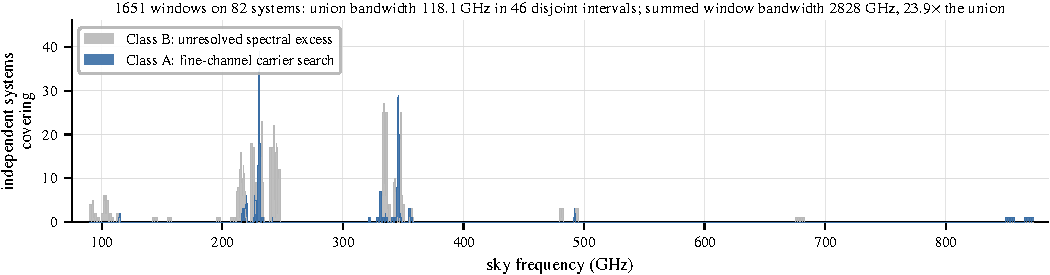
\includegraphics[width=0.99\textwidth]{figures/coverage_waterfall.pdf}
\caption{Where this survey searched. \emph{Lower panel:} each searched
window is a horizontal segment on its host system's row, rows ordered by
distance and labelled alternately on the left and right axes; heavy blue
marks the fine-channel carrier search (Class~A) and light grey the
coarse-channel spectral-excess search (Class~B). \emph{Upper panel:} the number
of systems covering each gigahertz of sky frequency; the threshold
distribution is Fig.~\ref{fig:context}(a). The coverage is narrow and
repeatedly revisited: the summed window bandwidth is $\GrossOverUnion\times$
the union, so the union measures frequency coverage and the summed bandwidth
search effort.}
\label{fig:waterfall}
\end{figure*}

%% Floats that belong elsewhere: tab:blockledger is in Appendix A (its
%% headline rows are in the prose above, so the cross-reference is not a
%% pointer with no numbers beside it); tab:interesting is deposited row for
%% row rather than typeset; tab:searchspace is deleted, nothing having cited
%% it, and its counts, unions, channel widths and drift range are all
%% elsewhere in the paper.
%% Carried forward to the numbers owner: tab_interesting.tex is still
%% generated but is not in make_all.sh, and its planet column should read the
%% dated NASA Exoplanet Archive extract selfunc_v411.py uses so that one
%% definition of "confirmed planet" serves both tables.  Two display defects
%% belong in star_alias.designation: Barnard's Star prints as a SIMBAD
%% identifier with the "NAME" prefix stripped, and BD+05 1668 would read
%% better with its GJ alias beside it.
